\exercise

Given the tree $(1,2),\ (2,x),\ (2,y),\ (2,z),\ (1,3),\ (3,u),\ (3,v)$, of
internal nodes $\{ 1, 2, 3 \}$ and leaves $\{ x, y, z, u, v \}$, apply the
transformation \emph{Euler Tour} $\rightarrow$ \emph{Sparse Table} and
\emph{Prefix/Suffix Arrays} to answer in constant time lowest common ancestor
queries between pair of leaves.

\solution

\begin{figure}[b  ]
  \centering
  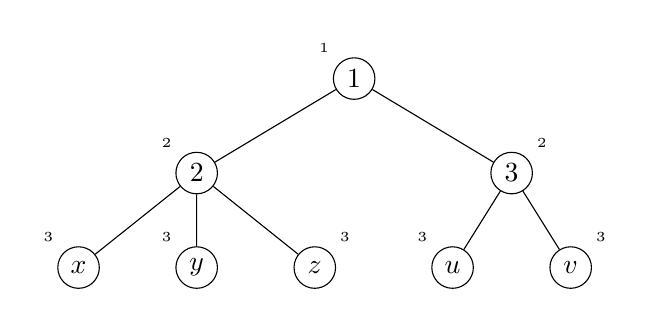
\begin{tikzpicture}[
    grow=down,
    every node/.style={draw, fill=white, inner sep=0, minimum size=15, circle},
    level 1/.style={sibling distance = 4cm, level distance = 1.2cm},
    level 2/.style={sibling distance = 1.5cm, level distance = 1.2cm}
  ]
  \node[label=135:{\tiny 1}] (1) {1}
  child {
    node[label=135:{\tiny 2}] (2) {2}
    child {
      node[label=135:{\tiny 3}] (x) {$x$}
      edge from parent[-]
    }
    child {
      node[label=135:{\tiny 3}] (y) {$y$}
      edge from parent[-]
    }
    child {
      node[label=45:{\tiny 3}] (z) {$z$}
      edge from parent[-]
    }
    edge from parent[-]
  }
  child {
    node[label=45:{\tiny 2}] (3) {3}
    child {
      node[label=135:{\tiny 3}] (u) {$u$}
      edge from parent[-]
    }
    child {
      node[label=45:{\tiny 3}] (v) {$v$}
      edge from parent[-]
    }
    edge from parent[-]
  };
  \end{tikzpicture}

  \caption{Graphical representation of the tree. The labels outside each node
  represents its depth.}

  \label{fig:tree-depths}
\end{figure}
%
\autoref{fig:tree-depths} represents the tree of the text. To compute the LCA of
two leaf nodes, we first have to build the following data structures:
%
\begin{enumerate}

  \item We compute the Euler Tour of the tree and, for each node store its depth
  in an array $D$ of size $2e + 1$, where $e$ is the number of edges of the
  tree. The values of the Euler Tour and the array $D$ are shown in
  \autoref{tab:euler-tour}. Both arrays will have size $O(e) = O(n)$.
  %
  \begin{table}[t]
    \centering
    \begin{tabular}{|r||c|c|c|c|c|c|c|c|c|c|c|c|c|c|c|c|}
      \hline
      Euler Tour & 1 & 2 & $x$ & 2 & $y$ & 2 & $z$ & 2 & 1 & 2 & $u$ & 2 & $v$ & 2 & 1 \\\hline
             $D$ & 1 & 2 & 3 & 2 & 3 & 2 & 3 & 2 & 1 & 2 & 3 & 2 & 3 & 2 & 1 \\\hline\hline
        $\Delta$ & \multicolumn{1}{c}{1} & \multicolumn{1}{c|}{$+$} &
                   \multicolumn{1}{c}{3} & \multicolumn{1}{c|}{$-$} &
                   \multicolumn{1}{c}{3} & \multicolumn{1}{c|}{$-$} &
                   \multicolumn{1}{c}{3} & \multicolumn{1}{c|}{$-$} &
                   \multicolumn{1}{c}{1} & \multicolumn{1}{c|}{$+$} &
                   \multicolumn{1}{c}{3} & \multicolumn{1}{c|}{$-$} &
                   \multicolumn{1}{c}{3} & \multicolumn{1}{c|}{$-$} &
                   \multicolumn{1}{c|}{1} \\\hline
           $M_1$ & \multicolumn{2}{c|}{1} & \multicolumn{2}{c|}{2} &
                   \multicolumn{2}{c|}{2} & \multicolumn{2}{c|}{2} &
                   \multicolumn{2}{c|}{1} & \multicolumn{2}{c|}{2} &
                   \multicolumn{2}{c|}{2} & \multicolumn{2}{c|}{1} \\
           $M_2$ & \multicolumn{2}{c|}{1} & \multicolumn{2}{c|}{2} &
                   \multicolumn{2}{c|}{2} & \multicolumn{2}{c|}{1} &
                   \multicolumn{2}{c|}{1} & \multicolumn{2}{c|}{2} &
                   \multicolumn{2}{c|}{1} & \multicolumn{2}{c|}{--} \\
           $M_3$ & \multicolumn{2}{c|}{1} & \multicolumn{2}{c|}{1} &
                   \multicolumn{2}{c|}{1} & \multicolumn{2}{c|}{1} &
                   \multicolumn{2}{c|}{1} & \multicolumn{2}{c|}{--} &
                   \multicolumn{2}{c|}{--} & \multicolumn{2}{c|}{--} \\\hline
    \end{tabular}

    \caption{The values of the Euler Tour, the depth array $D$, the pattern
    array $\Delta$ and the sparse table $M$. In \Delta, ``+'' represents an
    increment and ``--'' a decrement. The last element of $\Delta$ may be
    considered as an all-ascending block (i.e., $(1, +)$).}

    \label{tab:euler-tour}

  \end{table}

  \item We divide the array $D$ in blocks of $d = \left\lceil \frac{1}{2}\log_2
  e \right\rceil = 2$ elements. For each block $D_k$, we construct
  %
  \begin{itemize}

    \item the array $\Delta_k$, such that $\Delta_k[1] = D_k[1]$ and $\forall i
    = 2, \dots, d.\ \Delta_k[i] = D_k[i] - D_k[i] \in \{+1, -1\}$. This array
    will have size $O(e) = O(n)$;

    \item the sparse matrix $M$, with each row $i \in [1, \log_2 2e]$ defined as
    $M_{i, j} = \min_{k = 0, \dots, 2^i - 1} D[j + k]$. This matrix will have
    size $O(\frac{e}{\log e}\log\frac{e}{\log e}) = O(e) = O(n)$.

  \end{itemize}

  \item We construct a table $T$ for each triple $(i, j, p)$, where $i$ and $j$
  are indexes such that $1 \le i < j \le d$ and $p$ is a binary pattern such
  that $p \in \{+1, -1 \}^{d - 1}$. $T$ stores the position of the minimum in a
  given the range $[i, j]$ of a block $D_k$ having pattern $\Delta_k[2, d] = p$.
  The first value of $\Delta_k$ is not relevant for the computation of the
  \emph{position} of the minimum inside the block.  For this example, the values
  or $T$ are just the following
  %
  \begin{center}
    \begin{tabular}{c|c|c||c}
      $i$ & $j$ & $p$ & $T(i, j, p)$ \\\hline
      1 & 2 & $-1$ & 2 \\
      1 & 2 & $+1$ & 1 \\
    \end{tabular}
  \end{center}
  %
  The size of $T$ is $O(2^dd^2) = O(\sqrt{e}\log^2 e) = O(e) = O(n)$.

\end{enumerate}

Finally, to compute the LCA of two leaves $L$ and $R$, we proceed as follows:
%
\begin{enumerate}

  \item We retrieve the leftmost occurrence of $L$ and the rightmost occurrence
  of $R$ in the Euler Tour, respectively $l$ and $r$.

  \item If $l$ and $r$ are in the same block $D_k$, we compute $t = T(l - o, r -
  o, \Delta_k[2, d])$, where $o = dk$, and then get the position of the LCA in
  the Euler Tour with $t + o$.

  \item If $l$ and $r$ fall in two separate blocks, we first compute the minimum
  w.r.t. the blocks between the ones containing $l$ and $r$, by comparing
  $M_h[l]$ and $M_h[r - 2^h]$, with $h = \lfloor \log_2 (r - l)\rfloor$. Then we
  we retrieve the minimum for the blocks containing $l$ and $r$ by checking $T[l
  - o_L, d, \Delta_{k_L}]$ and $T[0, r - o_R, \Delta_{k_R}]$, with $o_L$ and
  $o_R$ defined as in the previous point. The overall minimum is found with a
  simple comparison.

\end{enumerate}
